\section{Аналитический раздел}
В соответствии с заданием на курсовой проект необходимо разработать программное обеспечение которое с помощью камеры отслеживает сигнал и эмитирует пользовательские действия компьютерной мыши. Пользователь с помощью специального устройства (трех цветного фонарика) или специальных цветных карточек формирует сигнал. Программное обеспечение должно обеспечить получение данных сигналов черех камеру и преобразовать их в действия пользователя.

\subsection{Анализ подходов к реализации}

\subsection{Загружаемы модули ядра Linux}
Ядро Linux относится к категории так называемых монолитных - это означает что большая часть функциональности опирационной сисетмы называется ядром и запускается в привилегированном режиме.
Этот подход отличен от подхода микроядра, когда в режиме ядра выполняется только основная функциональность (взаимодействия между процессами [inter-process communication, IPC], диспетчеризация, базовый ввод-вывод [I/O], управелние памятью), а остальная функциональность вытесняется за пределы привилегированной зоны (драйверы, сетевой стек, файловые системы). 
Можно было бы подумать, что ядро очень статично, но на самом деле все как раз наоборот. 
Ядро Linux динамически изменяемое - это означает, что вы можете загружать в ядро дполнительную функциональность, выгружать функции из ядра и даже добавлять новые модули, изпользующие другие модули ядра.
Преимущество загружаемых модулей заключается в возможности сократить расход памяти для ядра, загружая только необходимые модули (это может оказаться важным для встроенных систем) \cite{1}

Linux - не единственное динамически изменяемое монолитное ядро. Заружаемые модули поддерживаются в BSD-системах, Sun Solaris, а также в других популярных ОС, таких как Microsowft Windows и Apple Max OS X.

\subsubsection{Устройство модуля ядра}
Загружаемые модули ядра имеют ряд фундаментальных отличий от элементов интегрированных непосредственно в ядро, а также от обычнхы программ. Обычная программа содержит главную процедуру (main) в отличие от загружаемого модуля, содержащего функции входа и выхода (в версии 2.6 это функции можно наименовать как угодно). Функция входа вызывается когда модуль загружается в ядро, а функции выхода - соответсвенно при выгрузке из ядра.
Поскольку функции входа и выхода являются пользовательскими, для указания назначения этих функций используются макросы module\_init и module\_ext.
Загружаемый модуль содержит также набор обязательных и дополнительных макросов.
Они определяют тип лицензии, автора и описение модуля, а так же другие параметры.
Пример заружеченого модуля приведен на рисунке \ref{fig:coreexample}

% TODO: \usepackage{graphicx} required
\begin{figure}[H]
	\centering
	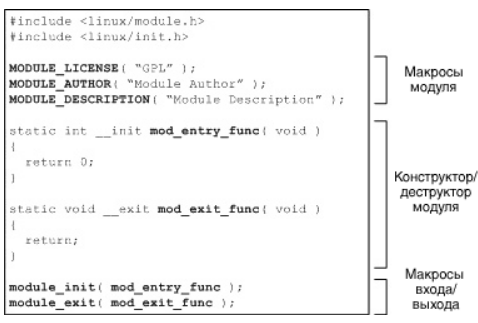
\includegraphics[width=0.7\linewidth]{src/img/core_example}
	\caption{Пример загружаемого модуля с разделами ELF}
	\label{fig:coreexample}
\end{figure}

\subsubsection{Анатомия объектного кода модуля ядра}
Загружаемый модуль представляет собой просто специальный объектный файл в формате ELF (Executable and Linkable Format). 
Обычно объектные файлы обрабатываются компоновщиком, который разрешает символы и формирует исполняемый файл. 
Однако в связи с тем, что загружаемый модуль не может разрешить символы до загрузки в ядро, он остается ELF-объектом. 
Для работы с загружаемыми модулями можно использовать стандартные средства работы с объектными файлами (которые в версии 2.6 имеют суффикс .ko, от kernel object). 
Например, если вывести информацию о модуле утилитой objdump, вы обнаружите несколько привычных разделов, в том числе .text (инструкции), .data (инициализированные данные) и .bss (Block Started Symbol или неинициализированные данные).

В модуле также обнаружатся дополнительные разделы, ответственные за поддержку его динамического поведения. 
Раздел .init.text содержит код module\_init, а раздел .exit.text – код module\_exit code. \ref{fig:coreelf}
Раздел .modinfo содержит тексты макросов, указывающие тип лицензии, автора, описание и т. д.

% TODO: \usepackage{graphicx} required
\begin{figure}[H]
	\centering
	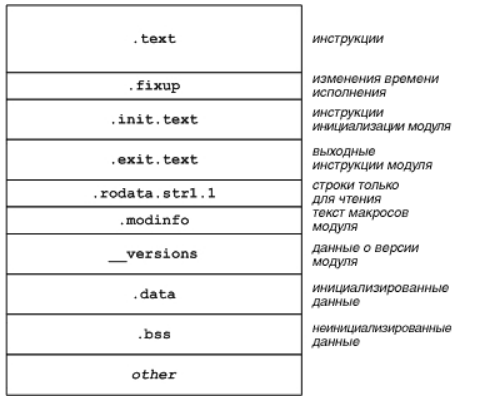
\includegraphics[width=0.7\linewidth]{src/img/core_elf}
	\caption{Пример загружаемого модуля с разделами ELF}
	\label{fig:coreelf}
\end{figure}

\subsubsection{Жизненный цикл загружаемого модуля ядра}
Процесс загрузки модуля начинается в пользовательском пространстве с команды insmod (вставить модуль). 
Команда insmod определяет модуль для загрузки и выполняет системный вызов уровня пользователя init\_module для начала процесса загрузки. 
Команда insmod для ядра версии 2.6 стала чрезвычайно простой (70 строк кода) за счет переноса части работы в ядро. 
Команда insmod не выполняет никаких действий по разрешению символов (вместе с командой kerneld), а просто копирует двоичный код модуля в ядро при помощи функции init\_module; остальное делает само ядро.

Функция init\_module работает на уровне системных вызовов и вызывает функцию ядра sys\_init\_module \ref{fig:commandsfunctions}. Это основная функция для загрузки модуля, обращающаяся к нескольким другим функциям для решения специальных задач. Аналогичным образом команда rmmod выполняет системный вызов функции delete\_module, которая обращается в ядро с вызовом sys\_delete\_module для удаления модуля из ядра.

% TODO: \usepackage{graphicx} required
\begin{figure}[H]
	\centering
	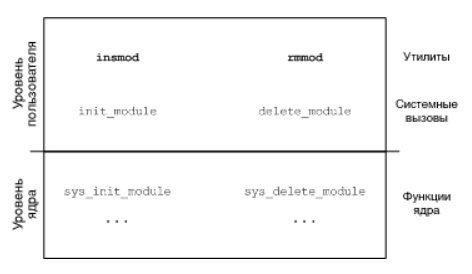
\includegraphics[width=0.7\linewidth]{src/img/commands_functions}
	\caption{Оновные команды и функции, участвуюие в загрузке и выгрузке модуля}
	\label{fig:commandsfunctions}
\end{figure}

Во время загрузки и выгрузки модуля подсистема модулей поддерживает простой набор переменных состояния для обозначения статуса модуля. 
При загрузке модуля он имеет статус MODULE\_STATE\_COMING. Если модуль загружен и доступен, его статус – MODULE\_STATE\_LIVE. Если модуль выгружен – MODULE\_STATE\_GOING.

\subsubsection{Подробности загрузки модуля}
Теперь давайте взглянем на внутренние функции для загрузки модуля \ref{fig:sysinitmodule}. 
При вызове функции ядра sys\_init\_module сначала выполняется проверка того, имеет ли вызывающий соответствующие разрешения (при помощи функции capable). 
Затем вызывается функция load\_module, которая выполняет механическую работу по размещению модуля в ядре и производит необходимые операции (я вскоре расскажу об этом). 
Функция load\_module возвращает ссылку, которая указывает на только что загруженный модуль. 
Затем он вносится в двусвязный список всех модулей в системе, и все потоки, ожидающие изменения состояния модуля, уведомляются при помощи специального списка. 
В конце вызывается функция init() и статус модуля обновляется, чтобы указать, что он загружен и доступен.

% TODO: \usepackage{graphicx} required
\begin{figure}[H]
	\centering
	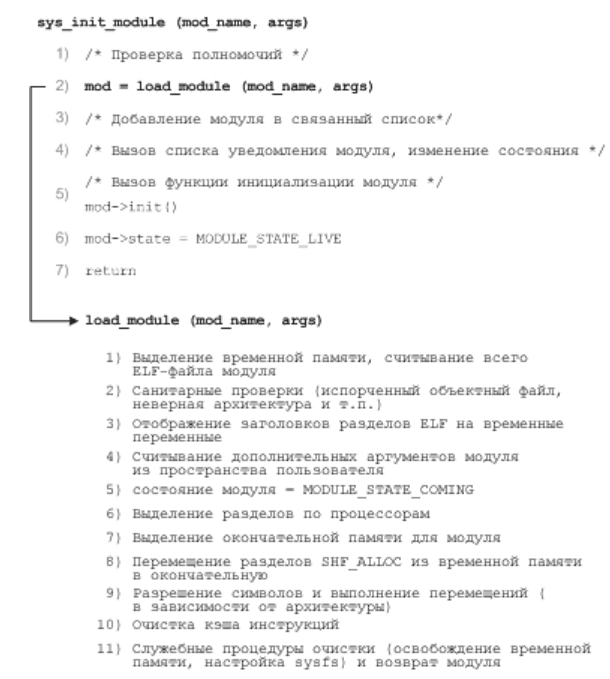
\includegraphics[width=0.7\linewidth]{src/img/sys_init_module}
	\caption{Внутренний процесс загрузи модуля (упрощенный)}
	\label{fig:sysinitmodule}
\end{figure}

Внутренние процессы загрузки модуля представляют собой анализ и управление модулями ELF. 
Функция load\_module (которая находится в ./linux/kernel/module.c) начинает с выделения блока временной памяти для хранения всего модуля ELF. 
Затем модуль ELF считывается из пользовательского пространства во временную память при помощи copy\_from\_user. 
Являясь объектом ELF, этот файл имеет очень специфичную структуру, которая легко поддается анализу и проверке.

Следующим шагом является ряд "санитарных проверок" загруженного образа (является ли ELF-файл допустимым? соответствует ли он текущей архитектуре? и так далее). 
После того как проверка пройдена, образ ELF анализируется и создается набор вспомогательных переменных для заголовка каждого раздела, чтобы облегчить дальнейший доступ к ним. 
Поскольку базовый адрес объектного файла ELF равен 0 (до перемещения), эти переменные включают соответствующие смещения в блок временной памяти. 
Во время создания вспомогательных переменных также проверяются заголовки разделов ELF, чтобы убедиться, что загружаемый модуль корректен.

Дополнительные параметры модуля, если они есть, загружаются из пользовательского пространства в другой выделенный блок памяти ядра (шаг 4), и статус модуля обновляется, чтобы обозначить, что он загружен (MODULE\_STATE\_COMING). 
Если необходимы данные для процессоров (согласно результатам проверки заголовков разделов), для них выделяется отдельный блок.

В предыдущих шагах разделы модуля загружались в память ядра (временную), и было известно, какие из них используются постоянно, а какие могут быть удалены. 
На следующем шаге (7) для модуля в памяти выделяется окончательное расположение, и в него перемещаются необходимые разделы (обозначенные в заголовках SHF\_ALLOC или расположенные в памяти во время выполнения). 
Затем производится дополнительное выделение памяти размера, необходимого для требуемых разделов модуля. 
Производится проход по всем разделам во временном блоке ELF,, и те из них, которые необходимы для выполнения, копируются в новый блок. 
Затем следуют некоторые служебные процедуры. 
Также происходит разрешение символов, как расположенных в ядре (включенных в образ ядра при компиляции), так и временных (экспортированных из других модулей).

Затем производится проход по оставшимся разделам и выполняются перемещения. Этот шаг зависит от архитектуры и соответственно основывается на вспомогательных функциях, определенных для данной архитектуры.
В конце очищается кэш инструкций (поскольку использовались временные разделы .text), выполняется еще несколько служебных процедур (очистка памяти временного модуля, настройка sysfs) и, в итоге, модуль возвращает load\_module.

\subsection{Подробности выгрузки модуля}
Выгрузка модуля фактически представляет собой зеркальное отражение процесса загрузки за исключением того, что для безопасного удаления модуля необходимо выполнить несколько "санитарных проверок". Выгрузка модуля начинается в пользовательском пространстве с выполнения команды rmmod (удалить модуль). 
Внутри команды rmmod выполняется системный вызов delete\_module, который в конечном счете инициирует sys\_delete\_module внутри ядра (вернитесь к рисунку \ref{fig:commandsfunctions}). Основные операции удаления модуля показаны на рисунке \ref{fig:uloadcore}.

% TODO: \usepackage{graphicx} required
\begin{figure}[H]
	\centering
	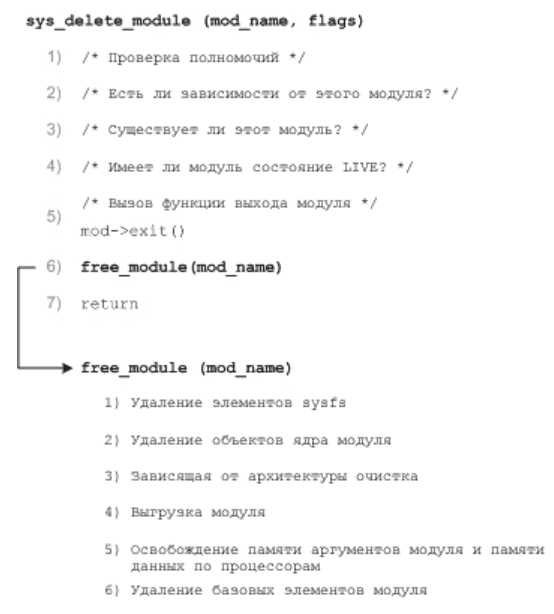
\includegraphics[width=0.7\linewidth]{src/img/uload_core}
	\caption{Внутренний процесс выгрузки модуля (упрощено)}
	\label{fig:uloadcore}
\end{figure}

При вызове функции ядра sys\_delete\_module (с именем удаляемого модуля в качестве параметра) сначала выполняется проверка того, имеет ли вызывающий соответствующие разрешения. Затем по списку проверяются зависимости других модулей от данного модуля. 
При этом используется список modules\_which\_use\_me, содержащий по элементу для каждого зависимого модуля. 
Если список пуст, т.е. зависимостей не обнаружено, то модуль становится кандидатом на удаление (иначе возвращается ошибка). 
Затем проверяется, загружен ли модуль. 
Ничто не запрещает пользователю запустить команду rmmod для модуля, который в данный момент устанавливается, поэтому данная процедура проверяет, активен ли модуль. 
После нескольких дополнительных служебных проверок предпоследним шагом вызывается функция выхода данного модуля (предоставляемая самим модулем). 
В заключение вызывается функция free\_module.

К моменту вызова free\_module уже известно, что модуль может быть безопасно удален. 
Зависимостей не обнаружено, и для данного модуля можно начать процесс очистки ядра. 
Этот процесс начинается с удаления модуля из различных списков, в которые он был помещен во время установки (sysfs, список модулей и т.д.). 
Потом инициируется команда очистки, зависящая от архитектуры (она расположена в ./linux/arch/<arch>/kernel/module.c). 
Затем обрабатываются зависимые модули, и данный модуль удаляется из их списков. 
В конце, когда с точки зрения ядра очистка завершена, освобождаются различные области памяти, выделенные для модуля, в том числе память для параметров, память для данных по процессорам и память модуля ELF (core и init).



